\chapter{Relle Rekonstruktion}
\label{sec:real} 

%3D-Stereokalibrierung und Szenenrekonstruktion mit reellen Daten und Kameras gleicher Auflösung
Durch im Minimabeispiel durchgeführten Stereoanalyse steht das Grundgerüst für die Stereoanalyse mit realen Bilddaten. Der selbe Arbeitsprozess soll nun auch auf ein Realbeispiel mit Bildern zweier Kameras durchgeführt werden. Die exterenen Kameraparameter, werden in extern beschaffen. Über \textit{Matlab} wird für jede Kamera einzeln mit Hilfe der \textit{Single-camera-aclibration} App eine Kalibrierung durchgeführt. Da diese auch dei externen Parameter liefert, können diese später als Vergleich mit den eigens berechneten Parameter dienen. Im fortschreitenden Arbeitsprozess der Stereoanalyse, werden des öfteren ungereimtheiten im Verlgeich mit dem Minimalbeispiel auftreten, welche behoben werden müssen um weiter zu verfahren. Diese Fehler entstehen durch die Ungenauigkeit, der zuvor detektierten korrespondierenden Punkte oder durch Bildfehler wie rauschen oder unschärfe, welche in der Fotographie nicht immer vermeiden werden können. Um diese Fehler zu beheben, werden einige zwischenschritte benötigt, welche im Minimalbeispiel durch die Reinheit der Daten und der selbst aufgebauten Szenen nicht nötig waren. Im Minimalbeispiel wurden einige solcher möglichen Fehler bereits erwähnt. Für die Stereoaufnahmen wurden die halbformat Kamera Canon 60 D und die Vollformatkamera 6D verwendet. Die Bilder wurden mit beiden Kameras mit selber Auflösung und Seitenverhältnis augenommen. Später wurden auch noch aufnahmen mit unterschiedlichen Auflösungen gemacht und ebenfalls die Stereoanalyse auf die Bildpaare angewandt.  \\

%Workflow beschreiben, hier die unterschiedlichen Starts zur Sprache bringen, also zum einen korrespondenz analyse mit schachbrett und eigenenem Algorithmus(Genauer Aufgeführt in Kapitel ....) und finden von Points of interest mit Hilfe des in mathematica vorprogrammierten SURF Verfahrens.\\
%
%Kameramatrizen werden extern über die Single Camera calibration app von Matlab herbeigezogen .
%
%Hier irgendwie überleiten, dass die Arbeit mit reelen Bilddaten einige komplexere zwischenschritte BEdingt auf Grund Bildfehler wie rauschen oder unschärfe der Bilde selbst. \\
%
%
%
%	Bis jetzt haben wir eine Stereoanalyse und Szenenrekonstrukion in einem wie wir es nennen Minimalbeispiel durchgeführt. Hierzu wurde zum Beispiel ein Quaderobjekt definiert und dessen Eckpunkte mit Hilfe von zwei selbst definierten Kameramatrizen verrechnet so, dass ein Stereobildpaar dieses Quaders entstand. \\
%	
%	
%	Vorteil war, dass man die korrespondierenden Punkte somit bereits besaß und die Stereoanalyse und Szenenrekonstruktion ohne Fehlerquellen wie Beispielsweise Rauschen durchführen konnte.\\
%	
%	 In unserem Beispiel unter Realbedinungen, müssen zunächst die korrespondierenden Punkte des Stereobildpaares ausgemacht werden, was bis jetzt, nicht besonders präzise, von Hand funktioniert. Zu dieser Ungenauigkeit kommen dann auch noch Fehler wie Rauschen hinzu.\\
%	 
%	  Wie hiermit bis jetzt verfahren wird, wird in den einzelnen Schritten nochmal genauer Aufgeführt folgend beschrieben.  


\section{Arbeitsprozess}


Die beiden Kameras wurden so im Raum platziert, dass sie leicht zueinander hin gedreht waren. Da die Canon 60D eine halbformatkamera ist, wurde sie weiter hinten als die Canon 6D positioniert. Somit konnte ungefähr der selbe Bildausschnitt der Szene mit beiden Kameras aufgenommen werden. \\

\begin{figure}[!htb]
	\minipage{0.48\textwidth}
	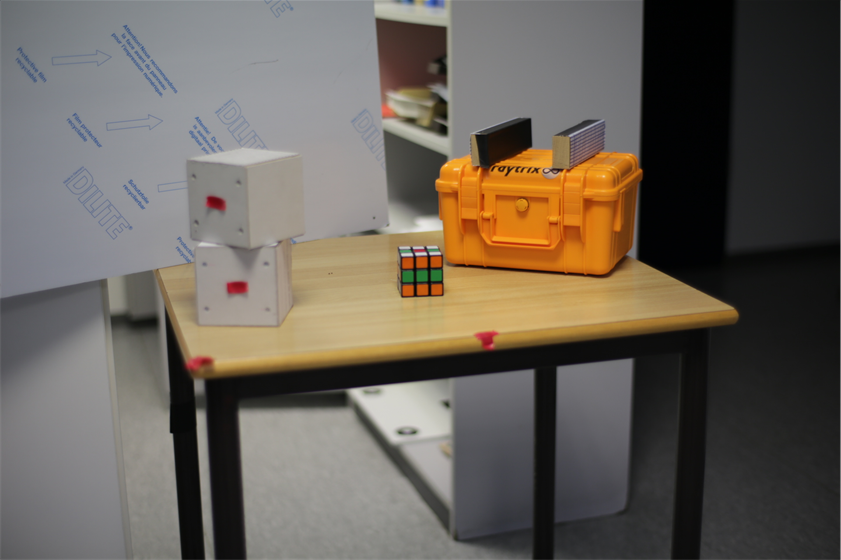
\includegraphics[width=\linewidth]{images/Points3DSceneLeft.png}
	\caption{Aufnahme der Canon 6D von links}
	\label{fig:awesome_image1}
	\endminipage\hfill
	\minipage{0.48\textwidth}
	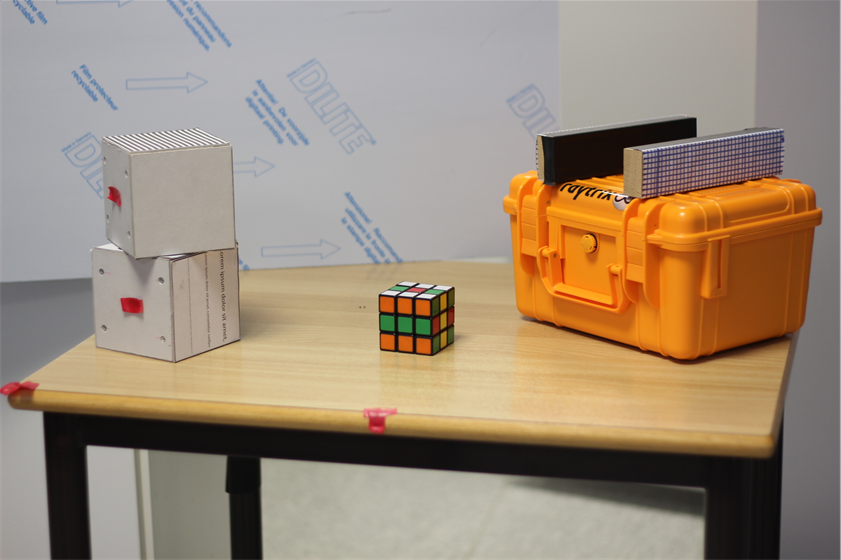
\includegraphics[width=\linewidth]{images/Points3DSceneRight.png}
	\caption{Aufnahme der Canon 60D von rechts}
	\label{fig:awesome_image2}
	\endminipage\hfill
\end{figure}

\begin{minipage}{\linewidth}
	\centering
	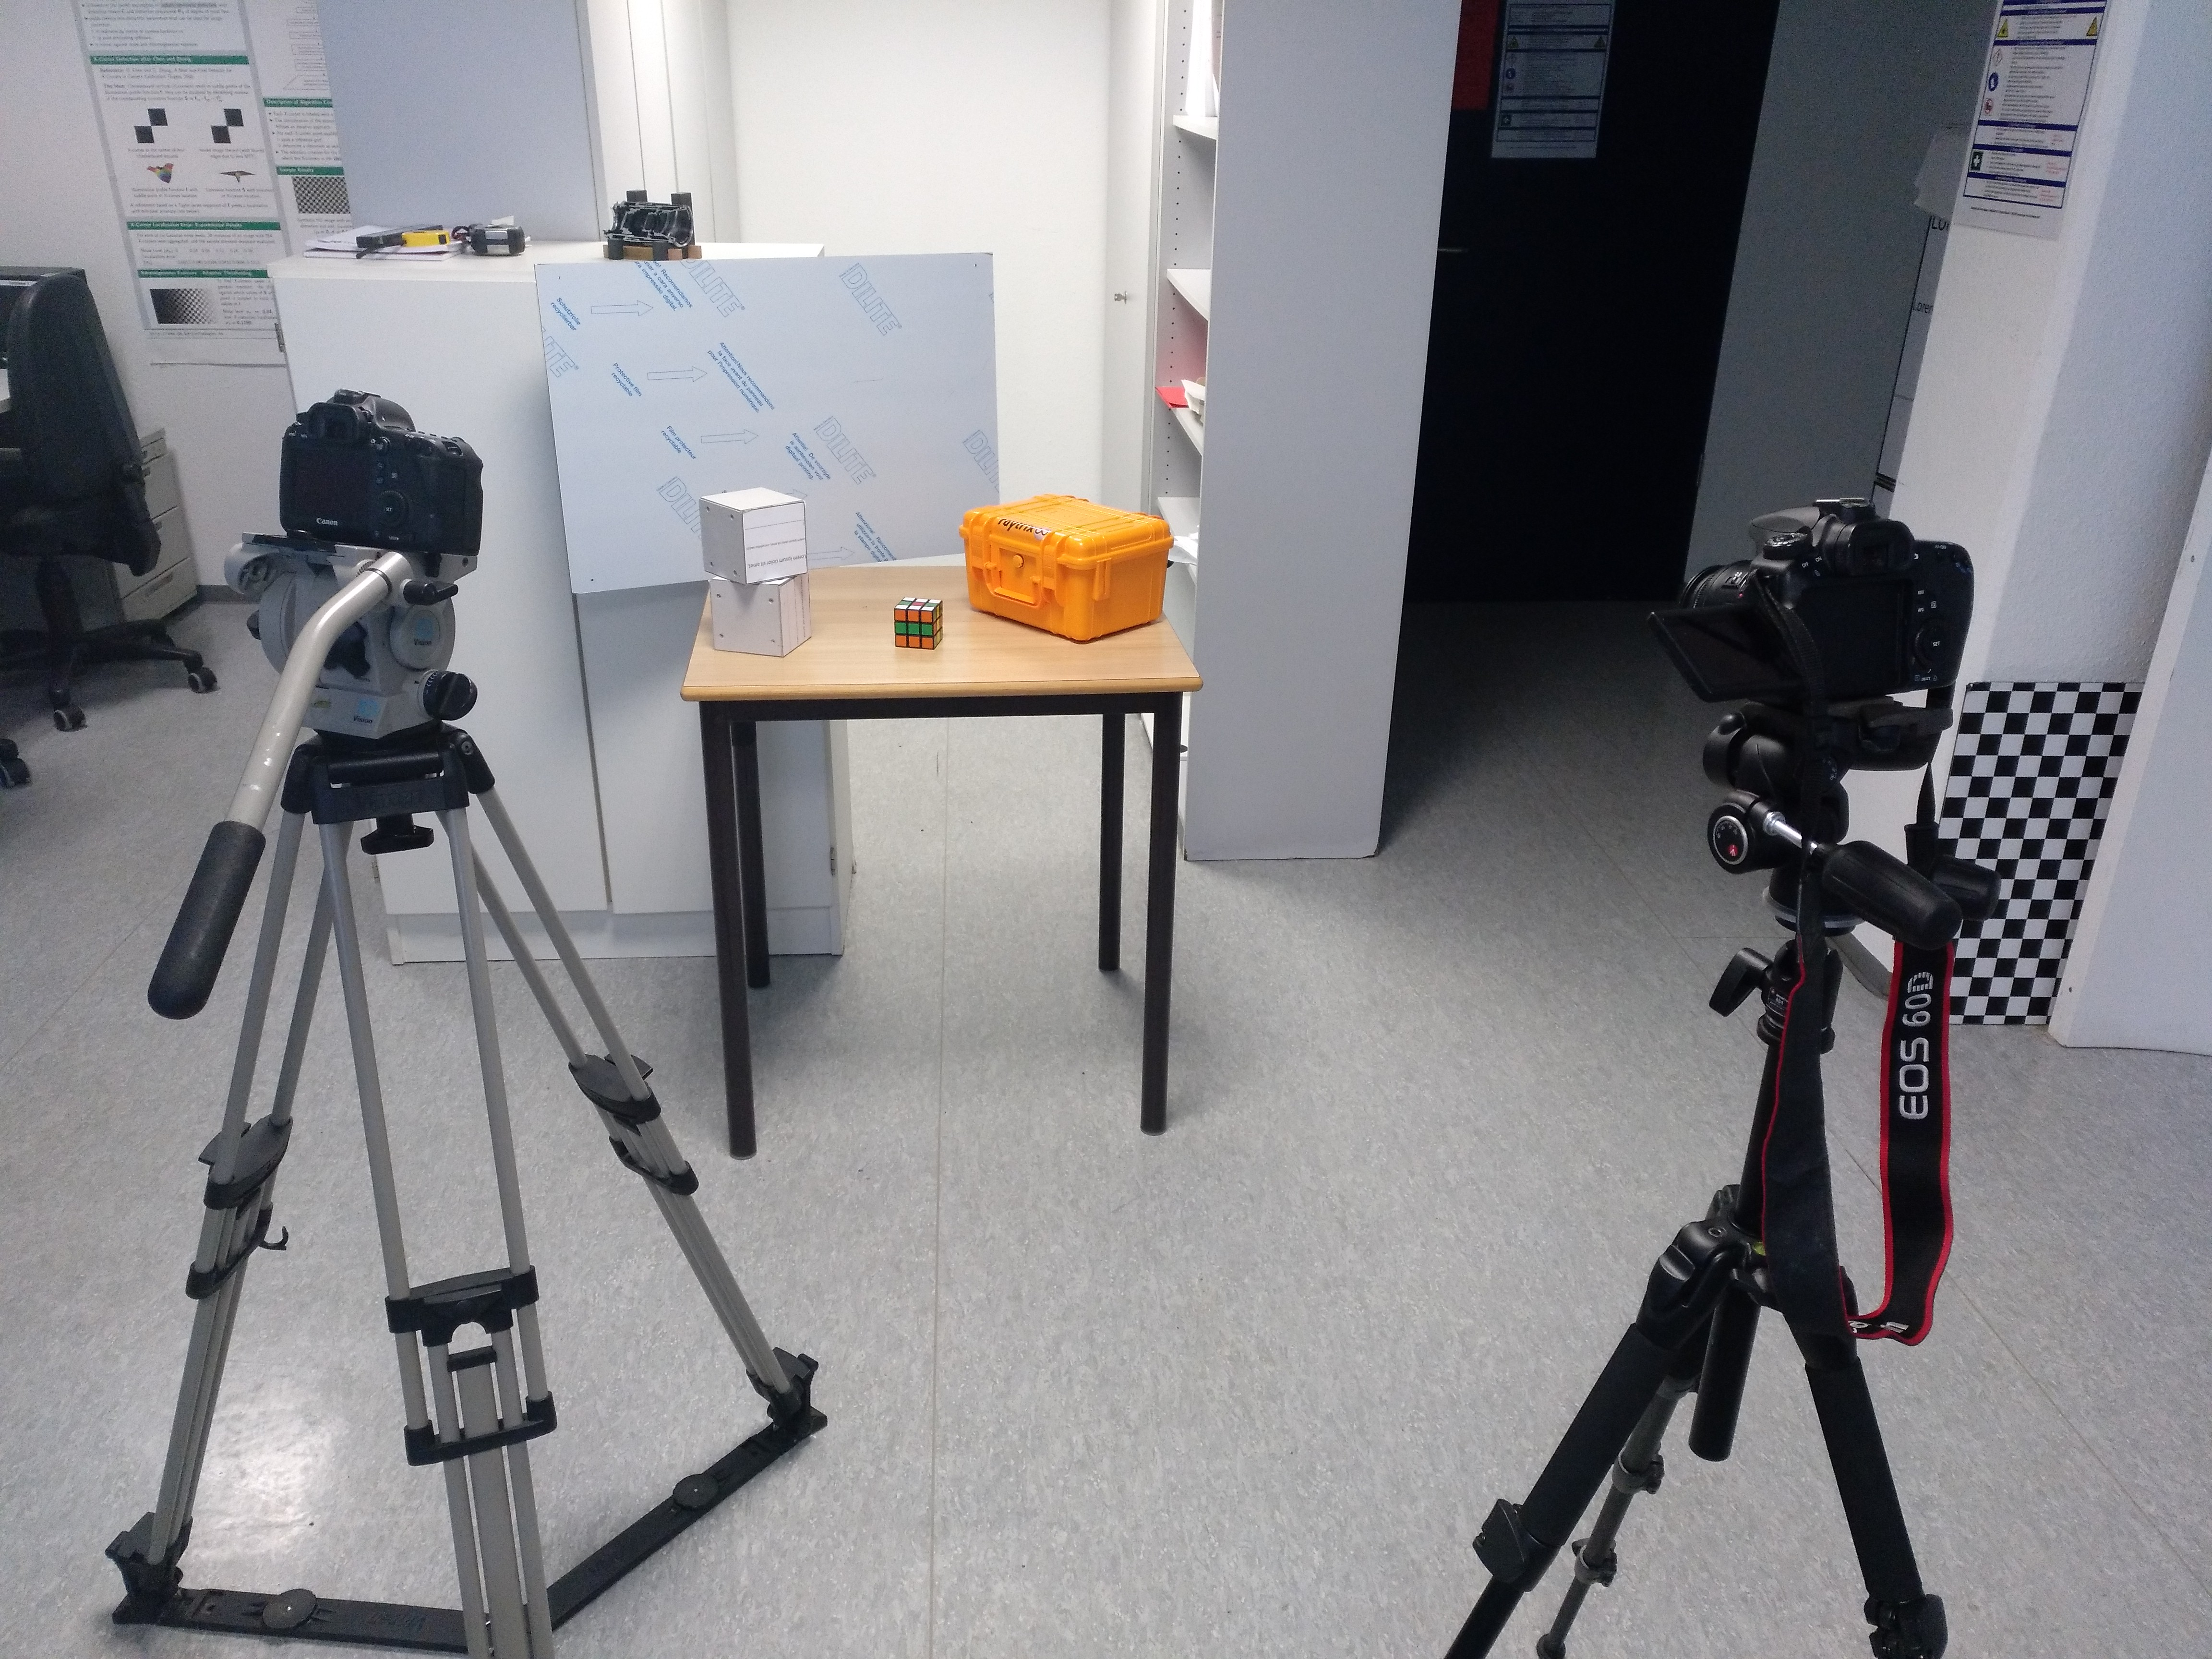
\includegraphics[width=.7\linewidth]{images/SetUpSameResolution.jpg}
	\captionof{figure}{Szenenaufbau: Die Canon 60D befindet sich in dieser Abbildung auf der linken Seite, die Canon 60 D auf der rechten. Auf dem Tisch zwischen den Kameras ist die in den Abbildungen 6.1 und 6.1 abgebildete Szene zu sehen. Die Canon 60D ist etwas hinter der Canon 6D positioniert. Beide Kameras sind zu Szene hin gedreht und auch leicht nach unten geneigt.}
\end{minipage}\\


Die Canon 6D wird als primär Kamera definiert und bekommt somit die bezeichnun $C$, während die Canon 60D ab jetzt mit $C'$ gekennzeichnet wird. Die räumliche Orientierung und Position von $C'$ wird also relativ zu $C$ berechnet und auch die Szene wird davon ausgehend, dass $C$ als Projektionsmatrix $P=[I|0]$ besitzt.

\begin{gather}
	P=\begin{pmatrix}
	I|0
	\end{pmatrix} =
	\begin{pmatrix}
	1&0&0&0\\
	0&1&0&0\\
	0&0&1&0
	\end{pmatrix}
\end{gather}\\

Die Koordinatensysteme von $C$ mit $(C, \beta)$ und das Weltkoordinatensystem $(O,\delta)$ werden deckungsgleich definiert. Das Koordinatensystem von $C'$ wird mit $(C', \beta')$ definiert. Für die spätere Skalierung der rekonstruierten Szene ist es ratsam innerhalb der Szene einen Abstand zweier Punkte zueinander abzumessen, um einen Referenzwert für die Skalierung zu bekommen. Der Stereoaufbau ist somit fertig installiert. Der nächste Schritt ist mit Hilfe von \textit{Matlab} und dem mitgelieferten Kalibrierungs-Tool namens \textit{Single-camera-calibration} für jede Kamera eine Kalibrierung durchzuführen, um so  die intrinsischen Parameter $K$ und $K'$ zu bekommen. Diese werden für den verwendeten Ansatz für die Schätzung der extrinsischen Parameter benötigt. Nach der Kalibrierung werden Stereoaufnahmen der Szene gemacht und anschließend korrespondierende Bildpunkte aus den beiden Bilder gesucht. Für den ersten Versuch wurden diese von Hand ausgelesen, da dies jedoch sehr Zeitaufwändig ist, wurden andere Möglichkeiten zur Detektion von korrespondierenden Bildpunkten überlegt. Wie in Abbildung (Einleitung Workflow) ersichtlich ist, wurde zwei Ansätze verfolgt. Fürs erste, wurde überlegt, ähnlich wie in \textit{Matlab} anhand von 2D Schachbrettern eine Stereoanalyse durchzuführen.\cite{MatlabStereoApp}. Ein 2D Schachbrett wird von beiden Kameras positioniert und es werden Stereoaufnahmen des selbigen gemacht. Mit Hilfe eines Algorithmus, welcher in einer vorherigen Arbeit angefertigt wurde, können die Eckpunkte des Schachbretts der jeweiligen Bilder bestimmt werden. Wichtig für die Funktion den Algorithmus ist, dass die Schachbretter vor einem einfarbigen Hintergrund aufgenommen wurden, so dass sich die Eckpunkt Bestimmung auch nur auf das Schachbrett bezieht und keine weiteren Punkte außerhalb mit in die entstehende Punkteliste aufgenommen werden. Wenn die Koordinatend der Eckpunkte des Schachbrettmusters bekannt sind, folgt ein weiterer Algorithmus, welcher im Zuge dieser Arbeit implementiert wurde. Dieser Algorithmus nimmt die Liste mit den Koordinaten der Eckpunkte entgegen und sortiert und nummeriert diese Zeilen- und Spaltenweise durch. Jeder Punkt ist somit über zwei Indizes codiert und enthält die Information, in welcher Zeile und in welcher Spalte des Schachbrettmusters er sich befindet. Dieser Algorithmus wird auf beiden Schachbrettern angewandt. Nach der Sortierung der Punkte auf beiden Bildern, ist es möglich, korrespondierende Punkte der Bilder anhand gleicher Indizes der Eckpunkte zu bestimmen. Da nicht immer garantiert ist, dass alle Punkte innerhalb des Schachbretts zuvor gefunden worden, enthält der Sortierungsalgorithmus eine Funktion, in welchem er Lücken des innerhalb ausfindig macht und synthetische Eckpunkte setzt. Diese synthetisch gesetzten Punkte, werden markiert, so dass sie nicht in die Liste der möglichen korrespondierenden Punkte fallen. Wie genau der Sortierungsalgorithmus implementiert wurde wird im Kapitel \nameref{sec:schachbrettAlg} genauer beschrieben. Danach wird wie in Abbildung ???(Einleitung) gezeigt weiter verfahren. Um eine 3D Szene rekonstruieren zu können, wurde mit Hilfe eines in \textit{Mathematica} bereits implementierten Verfahren zu Findung korrespondierender Punkte in zwei Bildern genutzt. Die benutzte Funktion basiert auf dem sogenannten \textit{SURF}-Algorithmus. \textit{SURF} steht für \textit{Speeded Up Robust Features} und ist ein Rotations- und Skaleninvarianter Punkte Detektor und Deskriptor\cite{SURF}. Die Suche nach diskreten Bildkorrespondenzen kann in drei Schritte eingeteil werden. Im ersten Schritt werde sogennaten \textit{Point of interest} an markanten Stellen im Bild detektiert. Darunter fallen zum Beispiel Eckpunkte-Erkennung, ''Blob''- Erkennung oder  ''T-Junctions''- Erkennung\cite{SURF}. Diese Aufgabe wird dem Detektor zugeordnet. Der wohl am meisten genutzte Detektor in heutigen Computer Vision Applikationen ist der sogenannte \textit{Harris corner detector}\cite{SURF}. Die Umgebung eines jeden gefundenen Punktes wird durch einen Merkmalsvektor beschrieben, den Deskriptor\cite{SURF}. Dieser Deskriptor muss unverwechselbar und zu gleichen Zeit robust  gegenüber Bildrauschen, Detektionsfehlern und geometrischen Deformationen sein. Im letzten Schritt müssen die Deskriptoren zwischen den Bildern abgestimmt werden. Meistens wird dieses \textit{matching} über die Distanzen der Vektoren betrieben. In Abbildung 6.4 ist eines der Ergebnisse des verwendeten \textit{SURF}-Algorithmus zu sehen. Das linke Bild wurde mit der Canon 6D aufgenommen, das rechte mit der Canon 60D. Die gelben Ziffern in den Bildern markieren die jeweiligen korrespondiernden Punkte in den Bildern.\\

\begin{figure}[!htb]
	\minipage{0.48\textwidth}
	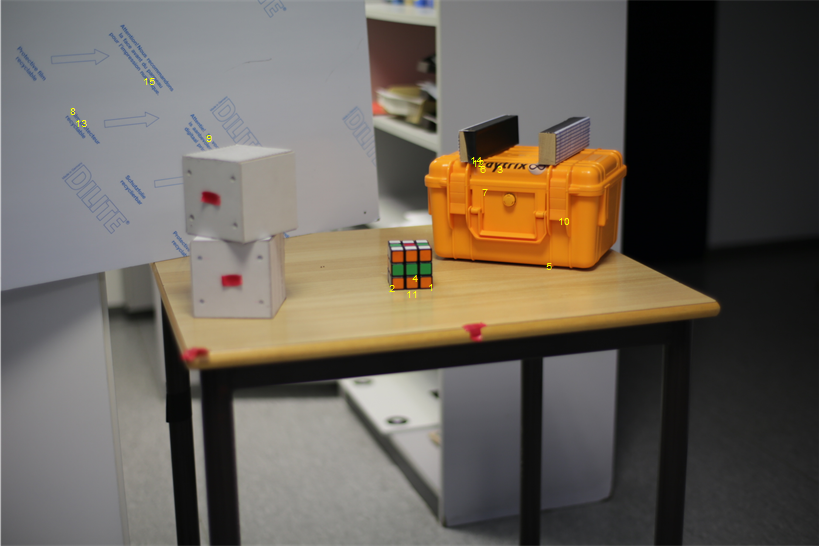
\includegraphics[width=\linewidth]{images/PointsDetectedLeft.png}
%	\caption{}
	\label{fig:awesome_image1}
	\endminipage\hfill
	\minipage{0.48\textwidth}
	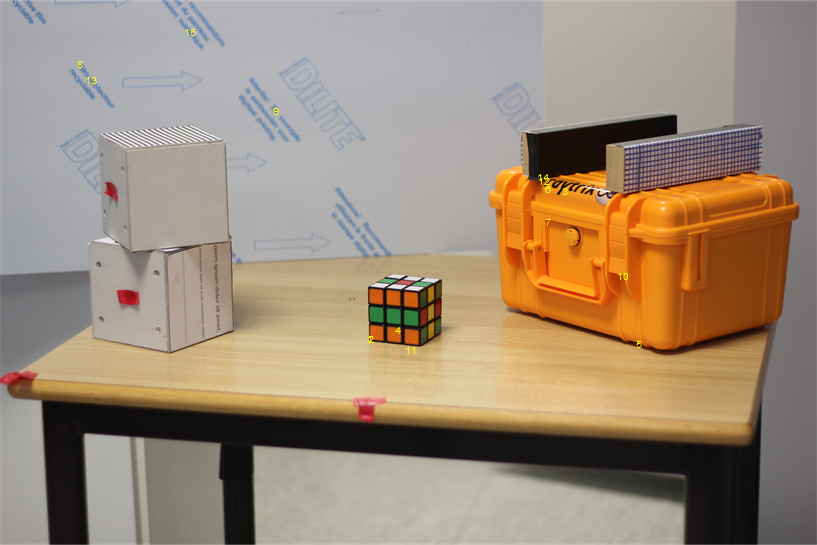
\includegraphics[width=\linewidth]{images/PointsDetectedRight.png}
%	\caption{Aufnahme der Canon 60D von rechts}
	\label{fig:awesome_image2}
	\endminipage\hfill
	\caption{Die mit dem \textit{SURF}-Algorithmus gefundenen Punkte sind mit den gelben Ziffern im Bild gekennzeichnet}
\end{figure}


\section{Normalized-eight-Point-Algorithm}

Nachdem die korrespondierenden Punkte in den Bilder gefunden wurden, wird nun der Arbeitsprozess wie in den Abbildungen ??? und ??? in der Einleitung und wie bereits aus dem Minimalbespiel bekannt, weiterverfolgt. In den einzelnen Schritten müssen jedoch ein paar Änderungen vorgenommen werde, um die durch die ungenauen Bilddaten entstehenden Fehler im Verlauf des Arbeitsprozesses zu minimieren. 

Als erstes erfolgt die Schätzung der Fundamentalmatrix. Für die Schätzung wurde eine leicht abgeänderte Form des \textit{eight-point-algorithms} namens \textit{normalized-eight-point-algorithm} angewandt\cite{HZ,HZ8,Ferid}. Zur Durchführung des \textit{normalized-eight-point-algorithm} wird eine vorherige Normierung der eingehenden Bildpunkte pro Bild verlangt. Diese sollen so normiert werde, dass ihr durchschnittlicher Abstand zu ihrem den Koordiantenursprung verschobenenen Schwerpunktes $\sqrt{2}$ beträgt\cite{HZ,HZ8,Ferid}. Zu aller erst werden die jeweiligen Schwerpunkte der Punkte in den einzelnen Bildern gesucht und dieser dann in den jeweiligen Sensorkoordinatenursprung verschoben. Die Bildpunkte werden unter Beibehaltung ihres momentanen Abstandes zum Schwerpunkt mit verschoben. Danach werden die Anbständer der Bildpunkten zum Schwerpunkt so skaliert, dass der Durchschnittsabstand der Punkte zu Schwerpunkt $\sqrt{2}$ beträgt. Die so skalierten Bildpunkte befinden sich nun in einem deutlich kleineren Zahlenbereich von circa $-1$ bis $1$\cite{HZ,HZ8,Ferid}. Die transformation der Bilddpunkte für beide Bilder wird jeweils einer Matrix $T$ und $T'$ vollzogen. Diese Matrix ist wichtig, um nach dem schätzen einer auf den normalisierten Koordinaten basierten Fundamentalmatrix $\hat{F}$ wieder eine denormalisierte $F$ zu generieren. Die Normierung der Bildkoordinaten ist wichtig, um die Auswirkung der Bildfehler auf das Endergebnis zu minimieren.  Die Entscheidung den normalized-8-Point-Algorithm  zu benutzen fiel als festgestellt wurde, dass ohne vorherige Normalisierung der ausgelesenen Punkte es zu größeren Fehlern in den weiteren Berechnungen kam. Zur Erklärung dieser Fehler kann zum einen die \textit{Condition-Number} betrachten. Als \textit{Condition Number}, Kondition im deutschen, wird die Abhängigkeit der Lösung eines Problems von der Störung der Eingangsdaten beschrieben. Die Kondition lässt sich durch Bestimmung des kleinsten Eigenvektors der Matrixmultiplikation der Koeffizientenmatrix $A$ mit ihrer Transponierten $A^T$ herausfinden. Die Matrix $AA^T$ wird in die Matrizen $UDU^T$, wobei $U$ eine orthogonale und $D$ eine diagonale Matrix ist, zerlegt. Die diagonaleinträge von $D$ sind in einen nicht ansteigenden Reihenfolge, woraus resultiert, dass der kleinste Singulärwert von $D$ mit der letzten Spalte von $U$ korrespondiert und somit ist die letzte Spalte von $U$ gleich dem kleinsten Eigenvektor von $AAt$\cite{HZ8}. Wird angenommen, dass $AA^T$ eine 9 $\times$ 9- Matrix ist, so ergeben die Einträge $d_1/d_9$ die gesuchte \textit{Condition Number}. je größer die \textit{Condition-Number} ist, desto größer wirken sich auch kleinste Abweichungen, wie Bildrauschen, auf die Resultate aus. Da sich die original Bildkoordinaten in diesem Beispiel in einem Zahlenbereich von 0 bis 5478 befinden, sind auch die Werte innerhalb der Koeffizientenmatrix in einem sehr großen Zahlenbereich, was zu Folge hat, das schon kleinste Abweichungen in den Bilddaten, große Auswirkungen auf die daraus resultierende Fundamentalmatrix haben kann, in Bezug darauf, dass die Werte der Einträge innerhalb von $F$, sehr große Ungleichgewichte aufweisen. Anders im Fall von Normierten Koordinaten, deren Zahlen sich in einem Bereich zwischen circa -1 und 1 befinden.  

\begin{gather}
	F = \begin{pmatrix}
		10^{-4}&10^{-4}&10^{-2}\\
	10^{-4}	&10^{-4}&10^{-2}\\
		10^{-2}&10^{-2}&1
	\end{pmatrix}\\
	F = \begin{pmatrix}
	-10^{-9}&10^{-6}&-10^{-4}\\
	-10^{-7}&10^{-4}&10^{-3}\\
	10^{-4}&-10^{-3}&-10^{-2}
\end{pmatrix}
\end{gather}

Gleichung 6.2 zeigt schematisch was unter einer Gleichgewichtigen Fundamentalmatrix zu verstehen ist, welche bei einer sehr gereingen \textit{Condition-number} resultieren kann. Gleichung 6.3 wiederum zeigt schematisch das Resultat einer Ungleichgewichteten Fundamentalmatrix, dessen \textit{Condition-Number} sehr groß ausfällt\cite{HZ8}. Durch normieren der Bildkoordinaten, kann die \textit{Condition-Number} kleiner und damit einhergehend die entstehenden Fehler minimiert werden. Nachdem die Fundamentalmatrix aus den normierten Koordinaten geschätzt wurde, wird sie anschließend mit den beiden aufgestellten Matrizen $T$
und $T'$ wieder denormalisiert, so dass sie wieder als $epipolar-contraint$ zwischen die original Koordinaten geschallten werden kann. Für normierte Koordinaten $\hat{m}$ und $\hat{m}'$ gilt $\hat{m}'^T \cdot \hat{F} \cdot \hat{m} = 0$ und für die ursprünglichen Bildkoordinaten gilt, dass $m'^T \cdot T'^T \cdot \hat{F} \cdot T\cdot m = 0$ und somit wieder $m'^T \cdot F\cdot m = 0$ \cite{HZ,HZ8,Ferid}. Die Normierung der Koordinaten für die Verwendung des \textit{eight-point-algorithms} darf auf keinen Fall mit der Normierung der Koordinaten für die essentielle Matrix $E$ verglichen werden. Die Normierung der Koordinaten für die Schätzung von $F$, soll die Auswirkungen von Fehler auf die Resultate minimieren, während die Normierung der Koordinaten durch deren Verrechnung mit den Kameramatrizen $K$ und $K'$ dafür sorgt, dass daraus normierte Bildkoordinaten entstehen, dess Koordinatenursprung nicht mehr in einer Bildecke sondern in der Bildmitte sich befindet\cite{HZ}. Um zurück zum Arbeitsprozess zu kommen, sind die Koordinaten normiert, so wird der im Kapitel \nameref{sec:einleitung} aufgezeigte Verfahren zur Schätzung der Fundamentalmatrix gleichermaßen wie in den Gleichungen 4.29 bis 4.34 aufgebaut. Durch die möglichen Ungenauigkeiten wie Bildrauschen oder dem detektieren der korrespondierenden Punkte, ist der Rang der aufgestellten Koeffizientenmatrix $A$ in den meisten Fällen größer als acht, was bedeutet, dass hier nicht einfach der Kern mit $A\cdot f = 0$ gesucht werden kann, um eine Lösung zu finden. Im Falle eines höhren Ranges als 8 muss ein Verfahren, ähnlich wie dem, welches angewandt wurde um überbestimmte Systeme zu Lösen um eine Homographiematrix zu erhalten. Es wird also derjenige Vektor für $f$ gesucht, welcher $||A\cdot f||$ minimiert. Hierzu wird eine Singulärwertszerlegung von $A$ in $A  = UDV^T$ durchgeführt. die Lösung für $f$, welche $||A\cdot f||$ minimiert ist dann diejenige Spalte von $V^T$, welche mit dem kleinsten Singulärwert von $D$ korrespondiert. Da die Singulärwerte eine absteigende Reihenfolge besitzen, bildet die letzte Spalte von $V^T$ den Vektor $f$\cite{HZ}.\\


\subsection{Singularity-Constraint der Fundamentalmatrix}
\label{sec:realFun}

Die Fundamentalmatrix ist eine singuläre-Matrix und ist somit eine Matrix von Rang zwei. Die singularität der Fundamentalmatrix sorgt zum einen dafür das ihr rechter und linker Kern jeweils den Epipol des jeweilgen Bildes ergibt und die Epipolarlinien auch alle durch eben diese Epipole verlaufen. wird die Fundamentalmatrix durch eine Singulärwertszerlung von $A$ geschätzt, ist die Chance sehr hoch, dass das Ergebnis für $\hat{F}$ eine Matrix von Rang 3 ist. Sollte dies der Fall sein gehen die Epipolarlinien der Bilder nicht mehr durch genau einen Punkt, wie man in den Abbildungen 6.5 und 6.6 erkennen kann. Diese bilden Epipolarlinien in einem Stereobildpaar ab.\\

\begin{figure}[!htb]
	\minipage{0.48\textwidth}
	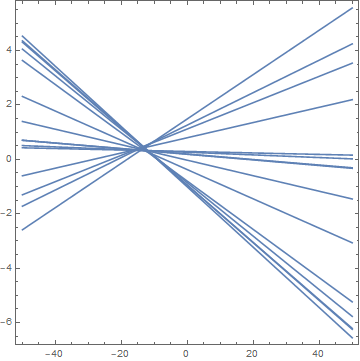
\includegraphics[width=\linewidth]{images/L_F_no_Constraint.png}
	\caption{Epipolarlinien ohne \textit{Epipolar-constraint} im Bild der Canon 6D}
	\label{fig:awesome_image1}
	\endminipage\hfill
	\minipage{0.48\textwidth}
	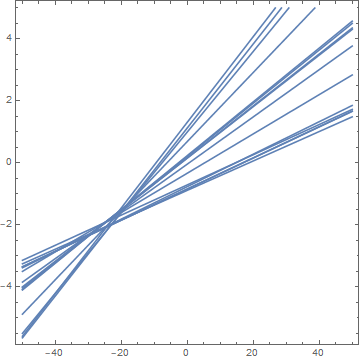
\includegraphics[width=\linewidth]{images/LPrime_PC2_F_no_Constraint.png}
	\caption{Epipolarlinien ohne \textit{Epipolar-constraint} im Bild der Canon 60D}
	\label{fig:awesome_image2}
	\endminipage\hfill
	%	\caption{Die mit dem \textit{SURF}-Algorithmus gefundenen Punkte sind mit den gelben Ziffern im Bild gekennzeichnet}
\end{figure}

Um eine gültige Fundamentalmatrix für den weiteren Arbeitsprozess zu generieren, kommt hier ein sogenannter \textit{singularity constraint} zum Einsatz. Dieser erzwingt in $\hat{F}$ eine Singularität. Zu aller erst wird eine Singulärwertszerlegung an $F$ durchgeführt, so dass $\hat{F}$ in $\hat{F} = UDV^T$ zerlegt wird. $D$ beinhaltet in einer diagonalen Matrix die Singulärwerte $D = \text{diag}(r,s,t)$, welche die Bedingung $r \leq s \leq t $ erfüllen. Um nun den \textit{singularity-constraint} in $\hat{F}$ zu erzwingen, wird der letzte Singulärwert $t = 0$ gesetzt, so dass am Ende dasteht $D = \text{diag}(r,s,0)$. Danach werden die Matrizen $UDV^T$, wobei $D$ nun die modifizierten Singulärwerte beinhaltet, wieder zu $\hat{F}$ multipliziert. Die jetzt resultierende Fundamentalmatrix $\hat{F}$ besitzt den Rang 2. Der rechte und linke Kern ergeben wieder die Epipole und die Epipolarlinien verlaufen wieder durch eben diese Epipole. Die Abbildungen 6.7 und 6.8 zeigen die selben Epipolarlinien wie in 6.5 und 6.6 nachdem der \textit{singularity-constraint} in $\hat{F}$ erzwungen wurde. Die somit entstandene Matrix $\hat{F}$, ist die laut Frobenius norm, nächste zum ursprünglichen $\hat{F}$\cite{HZ}.

Jetzt erst erfolgt die zuvor erwähnte denormierung von $\hat{F}$ durch $T$ und $T'$. Die Abbildungen 6.9 und 6.10 zeigen die Epipolarlinien im Originalbild mit denormierten Koordinaten.



\begin{figure}[!htb]
	\minipage{0.48\textwidth}
	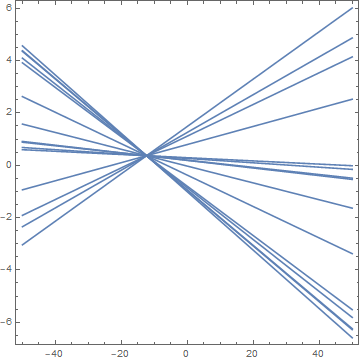
\includegraphics[width=\linewidth]{images/L_PC1_F_Constraint.png}
	\caption{Epipolarlinien mit \textit{Epipolar-constraint} im Bild der Canon 6D}
	\label{fig:awesome_image1}
	\endminipage\hfill
	\minipage{0.48\textwidth}
	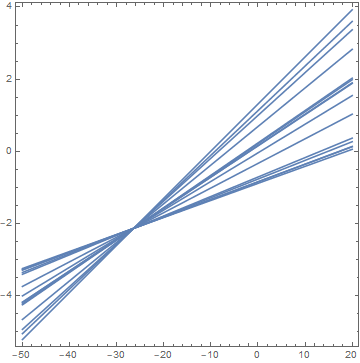
\includegraphics[width=\linewidth]{images/LPrime_PC2_F_Constraint.png}
	\caption{Epipolarlinien ohne \textit{Epipolar-constraint} im Bild der Canon 60D}
	\label{fig:awesome_image2}
	\endminipage\hfill
	%	\caption{Die mit dem \textit{SURF}-Algorithmus gefundenen Punkte sind mit den gelben Ziffern im Bild gekennzeichnet}
\end{figure}

\begin{figure}[!htb]
	\minipage{0.48\textwidth}
	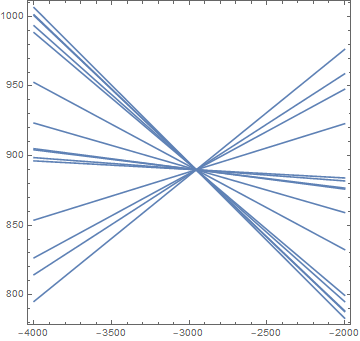
\includegraphics[width=\linewidth]{images/L_PC1_F_Constraint_denormalized.png}
	\caption{Epipolarlinien mit \textit{Epipolar-constraint} im Bild der Canon 6D, nach der denormalizierung von F}
	\label{fig:awesome_image1}
	\endminipage\hfill
	\minipage{0.48\textwidth}
	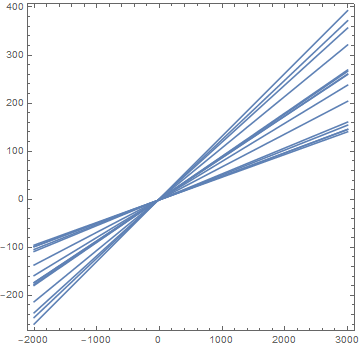
\includegraphics[width=\linewidth]{images/LPrime_PC2_F_Constraint_denormalized.png}
	\caption{Epipolarlinien ohne \textit{Epipolar-constraint} im Bild der Canon 60D, nach der denormalizierung von F}
	\label{fig:awesome_image2}
	\endminipage\hfill
	%	\caption{Die mit dem \textit{SURF}-Algorithmus gefundenen Punkte sind mit den gelben Ziffern im Bild gekennzeichnet}
\end{figure}

\pagebreak

\subsection{Singularity- Constraint der essentiellen Matrix}

Die essentielle Matrix $E$ kann wenn sie über den \textit{eight-point-algorithm} ermittelt wird, auch eine Rang 3 Matrix anstelle einer Rang 2 Matrix sein. Eine essentielle Matrix wird darüber definiert, dass sie eine Matrix mit Rang 2 ist und ihre Singulärwerte in $D$ von $E = UDV^T$ die Eigenschaft besitzen, dass $ D = diag(a,b,c)$ mit $a=b$ und $c=0$. Sind die Singulärwerte nicht in der gezeigten Form vorhanden und $E$ hat den Rang 3, so ist sie keine gültige essenetielle Matrix\cite{HZ}. Im implementierten Algorithmus, welcher in dieser Arbeit vorgestellt wird, wird die essentielle Matrix über die Fundamentalmatrix $F$ und den intrinsischen Kameraparameter $K$ und $K'$ gewonnen. Da im vorherigen Schritt für die Matrix $F$ schon der \textit{singularity-constraint} erwirkt wurde, ist dadurch dass $F$ nun eine MAtrix von Ran 2 ist auch versichert, dass $E$ ebenfalls von Rang 2 ist. Jedoch bedeutet das nicht gleichzeitig, dass auch die Bedingungen für die Singulärwerte von $E$ erfüllt sind. Wird $E$ in $UDV^T$ zerlegt und die Singulärwerte in D haben beispielsweise die Form $D= diag(a,b,c)$ mit $a \geq b \geq c $, so muss auch hier die für $E$ typische singularität erzwungen werden. Die laut Frobenuis Norm nächste Matrix $E$ zur momentanen $E$ kann durch modifizieren der Singulärwerte von $D$ mit $D=diag(\frac{a+b}{2},\frac{a+b}{2},0)$ erzwungen werden\cite{HZ}. Mit der neuen essentiellen Matrix können dann genau wie im Kapitel \nameref{sec:minimal} auch wieder die vier möglichen Lösungen der externen Kameraparameter ermittelt werden. 

\section{Szenenrekonstruktion}

Im letzten Schritt des Arbeitsprozesses, wird nun noch die Szenen mit Hilfe eines Triangulationsverfahrens rekonstruiert. Wie bereits im Kapitel \nameref{sec:minimal} erwähnt wurde, ist es bei den Fehlerhaften Bildkooridinaten nicht möglich die 3D-Szenenpunkte durch eine einfache Rückprojektion der der Bildpunkte zu einem Punkt im 3D-Raum zu erhalten. liegt nur einer der beiden Bildpunkte $m$ oder $m'$ nicht hundert prozentig auf der jeweilgen korrespondierenden Epipolarlinie, so liegen die rückprojizierten Strahlen windschief im Raum. Das liegt daran, dass die Bildpunkte $m$ und $m'$ nicht den \textit{Epipolar-Constraint} $m'^T F m = 0$ erfüllen. Sprich die Gleichungen $m = PM$ und $m' = P'M$ können nicht erfüllt werden, da es kein $M$ gibt, dass für beide Gleichungen mit den momentanen $m$ und $m'$ gibt. Abbildung 6.11 veranschaulicht die Rückprojektion der Kamerazentren durch zwei Fehlerhafte Bildpunkte. 

\begin{figure}[!htb]
	\minipage{0.48\textwidth}
	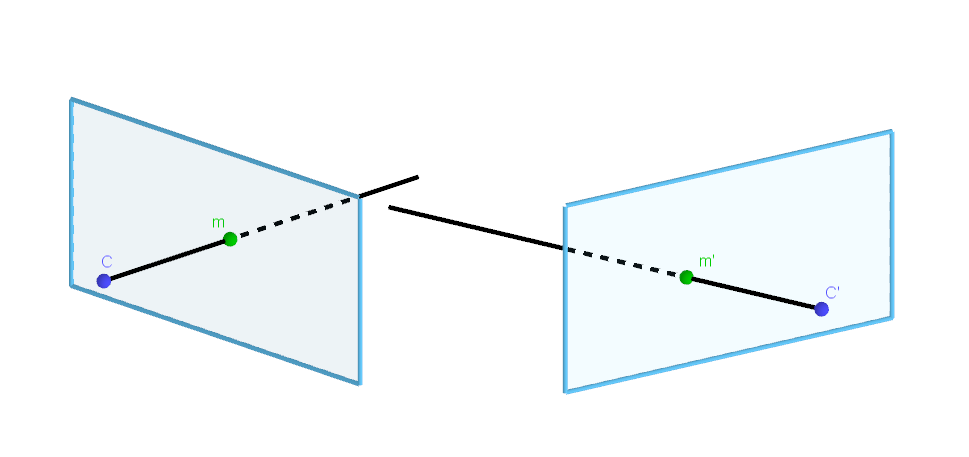
\includegraphics[width=\linewidth]{images/problemTriangulation.png}
	\caption{a)}
	\label{fig:awesome_image1}
	\endminipage\hfill
	\minipage{0.48\textwidth}
	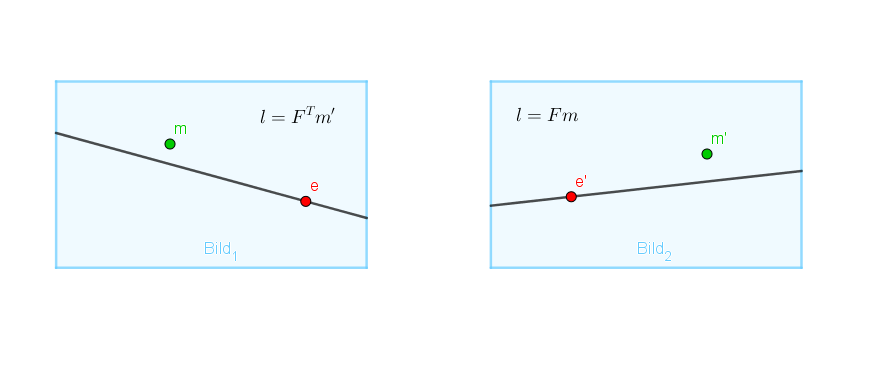
\includegraphics[width=\linewidth]{images/SampsAppx.png}
	\caption{b)}
	\label{fig:awesome_image2}
	\endminipage\hfill
	\caption{ a) Die rückprojzierten Strahlen der ungenauen korrespondierenden Punkte $m$ und $m'$ sind schief und treffen sich nicht in einem Punkt im 3D-Raum. b) The epipolar geometry for $m,\, m'$. The measured points do not satisfy the epipolar constraint.	The epipolar line $l' = Fm$ is the image of the ray through $n$, and $l = F^Tm'$ is the image of the ray through $m'$. Since the rays do not intersect, $m'$ does not lie on $l'$, and $m$ does not lie on $l$.}
\end{figure}

%\begin{minipage}{\linewidth}
%	\centering
%	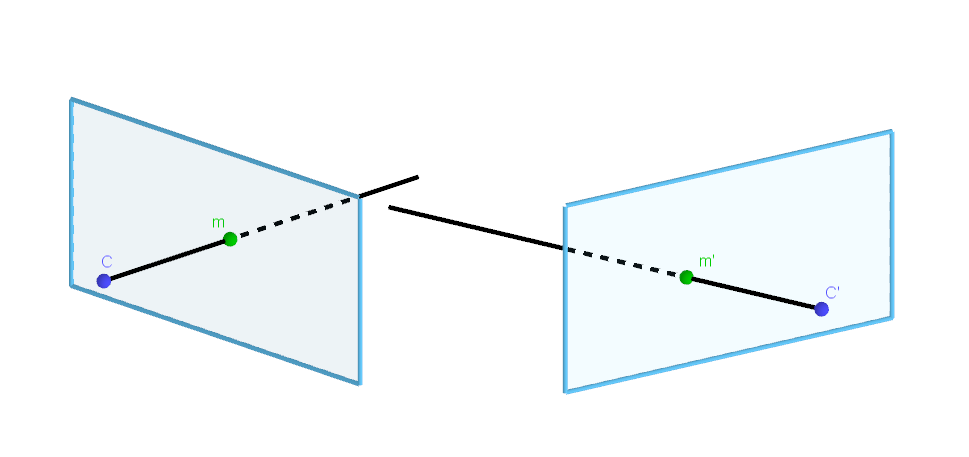
\includegraphics[width=.8\linewidth]{images/problemTriangulation.png}
%	\captionof{figure}
%\end{minipage}
%\begin{minipage}{\linewidth}
%	\centering
%	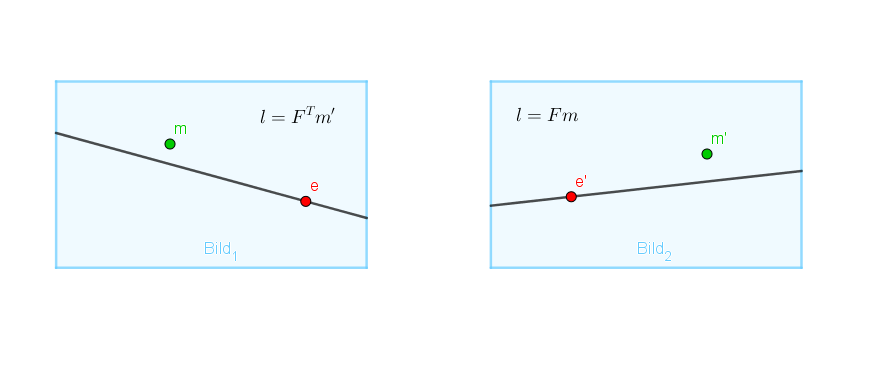
\includegraphics[width=.8\linewidth]{images/SampsAppx.png}
%	\captionof{figure}{The epipolar geometry for $m,\, m'$. The measured points do not satisfy the epipolar constraint.
%		The epipolar line $l' = Fm$ is the image of the ray through $n$, and $l = F^Tm'$ is the image of the ray through $m'$. Since the rays do not intersect, $m'$ does not lie on $l'$, and $m$ does not lie on $l$.}
%\end{minipage}

Um eine Triangulation zu ermöglichen, muss eine Methode gefunden werden, welche diesen Fehler so weit minimiert, dass es zu einer erfolgreichen Rückprojektion kommt. Die verwendete Methode zur Rekonstruktion der Szene wurde nach der Vorlage von \textit{Hartley \& Zisserman}\cite{HZ} implementiert und wird im folgenden Schritt für Schritt beschrieben. Voraussetzung ist, dass die Projektionsmatrizen $P$ und $P'$, sowie die Fundamentalmatrix $F$ bekannt sein müssen. Sind die Projektionsmatrizen $P$ und $P'$ bis auf eine projektive oder affine Komponenten bekannt, so ist es wünschenswert, wenn die Triangulierung auf einem affinen und projektiv invarianten Verfahren funktioniert\cite{HZ}. Die hier verwendeten Porjektionsmatrizen sind bis auf eine Skaleninvarianz genau bestimmt, was unter den Fall der affinen invarianz Fällt. Wären die intrinsischen Kameraparameter $K$ und $K'$ nicht bekannt gewesen, gibt es die Möglichkeit die Projektionsmatrizen über die Fundamentalmatrix $F$ mit dem, im Buch von \textit{Hartley \& Zisserman} beschriebenen  \textit{Stratified-Approach} bis auf eine projektive Invarianz genau zu bestimmen\cite{HZ}. Die hier verwendete Triangulierung ist nur projektiv invariant, kann aber trotzdem genutzt werde. Die rekonstruierte Szene ist, dann wie im Minimalbeispiel auch, nicht auf ihre Originalmaße skaliert, was aber nach der Triangulierung noch getan werden kann. Die Triangulierung ist deshalb projektiv invariant, weil alle Rechenoperationen, wie die Minimierungen von Distanzen, sich nur auf die 2D-Bildern bezihen und sich nicht in den projektiven 3D-Raum erstreckt\cite{HZ}. Der Grundgedanke der Triangulation ist, dass zwei Punkte $\hat{m}$ und $\hat{m'}$ gefunden werden sollen, die möglichst nah an den ursprünglichen $m$ und $m'$ sind und gleichzeitig den \textit{Epipolar-Constraint} $\hat{x}'^TF\hat{x} = 0$ erfüllen. Dies erfolgt durch die Minimierung einer Kostenfunktion $C$. In vielen bekannten Computer Vision Applikationen wird für diese Minimierung eine numerische Lösung gewählt, die wohl bekannteste Methode ist der \textit{Levenberg-Marquardt} Algorithmus\cite{HZ}. Jedoch hat sich gezeigt, dass ein nahezu optimales Minimum der geometrischen Kostenfunktion $C$ auch durch eine Annäherung ersten Grades finden lässt. Die Annährung um die es sich handelt ist die sogenannten \textit{Sampson-approximation}


\subsection{Minimieren der Kostenfunktion durch Sampson-approximation}
\label{sec:sampson}

Es sollen zwei Punkte $\hat{m}$ und $\hat{m}'$ gefunden werden, welche nahe an den Ursprünglichen $m$ und $m'$ liegen und gleichzeitig den \textit{Epipolar-Constraint} erfüllen. $\hat{m}$ und $\hat{m}'$ sollen durch Minimierung einer Kostenfunktion $C$ ermittelt werden, welche die Distanz  $d$ zwischen $m$ und $\hat{m}$ und $m'$ und $\hat{m'}$ minimiert.


\begin{gather}
	C(m,m') = d(m,\hat{m})^2 + d(m',\hat{m'})^2
\end{gather}

Die projizierten Punkte $\hat{m}$ und $\hat{m'}$ eines 3D-Objektpunktes $\hat{M}$ liegen auf einem paar korrespondierender Epipolarlinien. Jedes Punktepaar, welches den \textit{Epipolar-Constraint} erfüllt, liegt auf einem paar korrespondierender Epipolarlinien. Die optimalen $\hat{m}$ und $\hat{m'}$ liegen am Fuße des Lots, welches von den ursprünglich projizierten Punkten $m$ und $m'$ ausgeht. Zusätzlich liegen $\hat{m}$ und $\hat{m}'$ auf korrespondierenden Epipolarlinien $l$ und $l'$\cite{HZ}. 

\begin{minipage}{\linewidth}
	\centering
	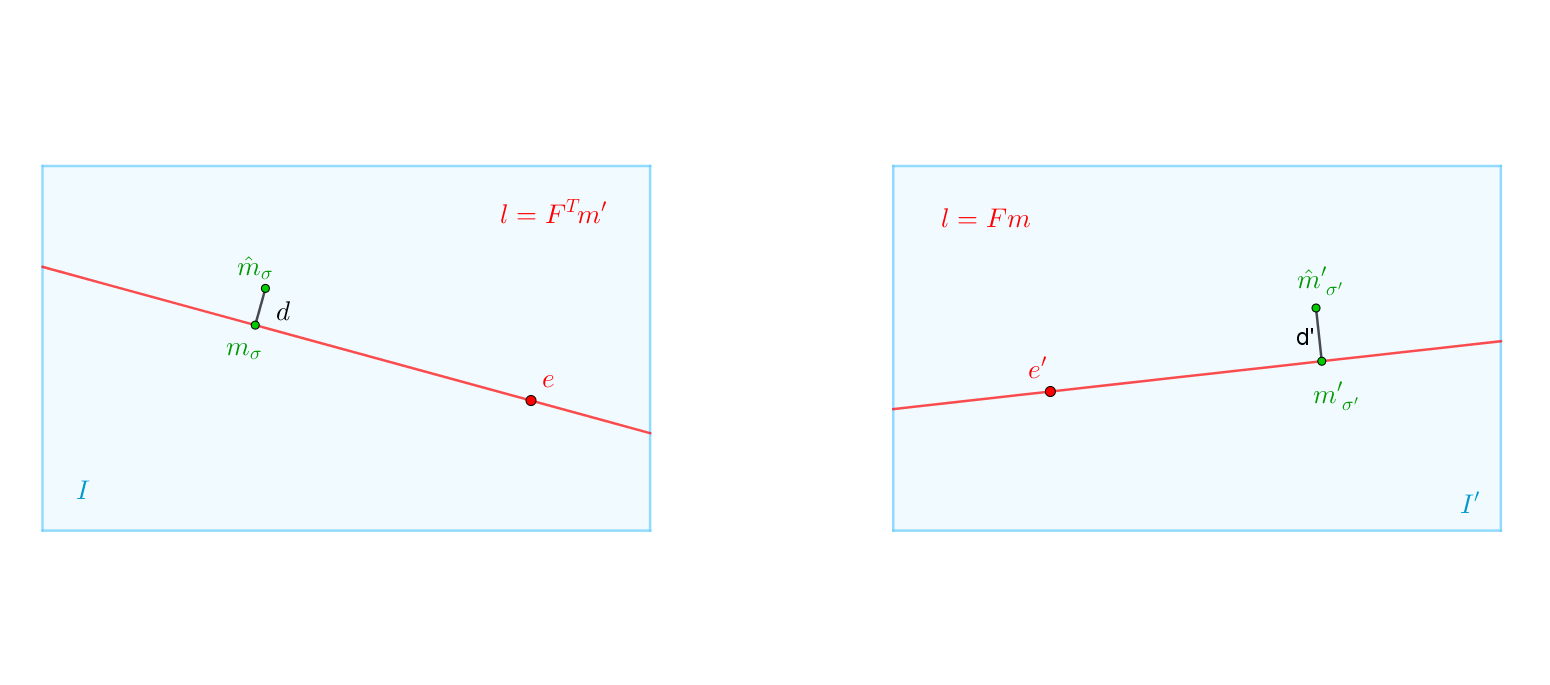
\includegraphics[width=.8\linewidth]{images/SampsAppxNewPoints.png}
	\captionof{figure}{Frafische Darstellung der optimalen Punkte $\hat{m}$ und $\hat{m'}$}
\end{minipage}\\

Jedes Punktepaar auf $l$ und $l'$ würde den \textit{Epipolar-Constraint} erfüllen, jedoch minimieren nur $x_\bot$ und $x'_\bot$ die quadratischen Distanzen in der Kostenfunktion $C$. Ausgehend von dieser Aussagen wird $C$ so umformuliert, d s gilt $d(m,\hat{m}) = d(\hat{m},l)$ und  $d(m',\hat{m}') = d(\hat{m}',l')$, was jeweils den senkrechten Abstand $m$ zu $l$ und $m'$ zu $l'$ beschreibt. Werden $l$ und $l'$ frei aus allen möglichen Epiploarlinien gewählt, so wird immer der senkrechte Abstand von $x$ zu dieser gewählten $l$ berechnet, entsprechend gilt das auch für $m'$ und irgendeine $l'$. Nun muss der Abstand $d(\hat{m},l)^2+ d(\hat{m}',l')$ minmiert werden, da natürlich nicht einfach jede beliebigen Epipolarlinien genutzt werden können. Es wird eine Strategie mit insgesamt vier Schritten für die Minimierung verfolgt\cite{HZ}. Zuerst werden die Epipipolarlinienbündel pro Bild so Parametrisiert, dass beispielsweise eine Epipolarlinie im ersten Bild als $l(t)$ geschrieben werden kann. Danach wird die Fundamentalmatrix $F$ dazu benutzt, die entsprechend korrespondierende Epiploarlinie $l'$ zu berechnen. Die Kostenfunktion $C$ kann somit als eine Funktion von $t$ definiert werden. Schlussendlich muss ein Wert für $t$ gefunden werden, welcher $C$ minimal werden lässt. 

\begin{gather}
	C(m,m') = d(m,\hat{m})^2 + d(m',\hat{m'})^2\\
	\leadsto 
	C(m,m') = d(m,l(t))^2 + d(m',l'(t))^2
\end{gather}\\

Es kann passieren , dass ein Bildpunkt korrespondierend zum jeweiligen Epipol des anderen Bildes ist, der Rückprojizierte Punkt im 3D-Raum würde sich dann auf der Basislinie der zwei Projektionszentren befinden und es ist somit nicht möglich ihn zu rekonstruieren. Um solche Fälle zu vermeiden, wird eine Transformation der Punkte $m$ und $m'$ in den Ursprung $(0,0,1)^T$ zu verschieben.

\begin{gather}
	T = \begin{bmatrix}
	1&0&-x\\
	0&1&-y\\
	0&0&1
	\end{bmatrix} \leadsto \bar{m} = T\cdot m\\
	T' = \begin{bmatrix}
	1&0&-x'\\
	0&1&-y'\\
	0&0&1
	\end{bmatrix} \leadsto 	\bar{m}' = T' \cdot m'
\end{gather} \\

Die Fundamentalmatrix $F$ wird dann wieder an die neu translatierten Punkte $\bar{m}$ und $\bar{m}'$ angepasst.

\begin{gather}
	\bar{F}= T'^{-T}FT^{-1}
\end{gather}

Als nächstes wird $F$ mit $T$ und $T$ so Transformiert, dass den \textit{Singularity-Constraint} zwischen 
Des Weiteren sollen die Epipole auf die x-Achse an die Punkte $\hat{e}=(1,0,f)^T$ und $\hat{e'}=(1,0,f')^T$, wobei $f$ und $f'$ nahezu null sein werden. Die Epipole lassen sich durch den rechten und linken Kern der neuen $\bar{F}$ berechnen. Angenommen $f$ und $f'$ seinen genau 0, so lauten die Koordinaten der Epipole $e = (1,0,f)^T$ und $e' = (1,0,f')^T$. Ist dies der Fall so hat $\bar{F}$ für welche dann gilt, dass $\bar{F}(1,0,f)^T = (1,0,f')\bar{F}=0$ eine spezielle Form.

\begin{gather}
	\bar{F} = \begin{pmatrix}
	ff'd&-f'c&-f'd\\
	-fb&a&b\\
	-fd&c&d
	\end{pmatrix}\\
	\begin{pmatrix}
	ff'd&-f'c&-f'd\\
	-fb&a&b\\
	-fd&c&d
	\end{pmatrix} \cdot \begin{pmatrix}
	1\\0\\f
	\end{pmatrix} = 
	\begin{pmatrix}
	ff'd + (-ff'd)\\
	-fb + fb\\
	-fd +fd
	\end{pmatrix}
	= 
	\begin{pmatrix}
	0\\0\\0
	\end{pmatrix}\\
	\begin{pmatrix}
	1&0&f'
	\end{pmatrix} \cdot
	\begin{pmatrix}
	ff'd&-f'c&-f'd\\
	-fb&a&b\\
	-fd&c&d
	\end{pmatrix} =
	\begin{pmatrix}
	ff'd + (-ff'd)\\
	-f'c + f'c\\
	-f'd + f'd
	\end{pmatrix} = 
		\begin{pmatrix}
	0&0&0
	\end{pmatrix}
\end{gather}

Im Realfall sind die Werte der Epipole $e$ und $e'$ nicht so rein wie im Beispiel gezeigt. Aufgrund dessen, werden zwei Rotationsmatrizen aufgestellt, welche die Epipole $e$ und $e'$ auf $Re = (1,0,e_3)$ und $R'e' = (1,0,e'_3)$ rotiert.

\begin{gather}
	R = \begin{bmatrix}
		e_1&e_2&0\\
		-e_2&e_1&0\\
		0&0&1
	\end{bmatrix}\\
	R' = \begin{bmatrix}
	e'_1&e'_2&0\\
	-e'_2&e'_1&0\\
	0&0&1
\end{bmatrix}
\end{gather}\\

$\bar{F}$ wird dann nochmals mit $R'FR^T$ ersetzt. Die Einträge in $\bar{F}_{Rot}$ haben nun die Form wie in Gleichung 7.10, mit $f = e_3, \, f' = e'_3, \, a = \bar{F}_{Rot,22}, \, b = \bar{F}_{Rot,23}, \, c = \bar{F}_{Rot,32}$ und $d = \bar{F}_{Rot,33}$. Angenommen eine Epipolarlinie verläuft nun durch einen Punkt $(0,t,1)^T$ und dem Epipol $e = (1,0,f)^T$, wird diese Epipolarlinie mit $l(t)$ bezeichnet. Das Kreuzprodukt dieser beiden Punkte beschreibt die Gerade. 

\begin{gather}
	\begin{pmatrix}
	0\\t\\1
	\end{pmatrix} \times
	\begin{pmatrix}
	1\\0\\f
	\end{pmatrix} = 
	\begin{pmatrix}
	tf\\1\\-t
	\end{pmatrix}
\end{gather}

Die quadratische Distanz dieser Linie zum Ursprung wird dann bezeichnet mit:


\begin{gather}
	d(m',l'(t))^2 = \frac{t^2}{1+(tf)^2}
\end{gather}

Für die Herleitung von Gleichung 7.16 wird angenommen die Gleichung einer Gerade sei zunächst in Koordinatenform Dargestellt 
\begin{gather}
	Ax+By-C = 0
\end{gather}

Die Selbe Gerade kann auch in Normalform ausgedrückt werden

\begin{gather}
\vec{n}\cdot (\vec{x} - \vec{p}) = 0\\
	\begin{pmatrix}
	A\\B
	\end{pmatrix}
	\cdot
	(\vec{x} - \vec{p}) = 0
\end{gather} 

Der Abstand eines Punktes zu einer Geraden kann folgend ausgedrückt werden.

\begin{gather}
	\vec{v} = \frac{\vec{p} \cdot \vec{n}}{\vec{n} \cdot \vec{n}} \cdot \vec{n}
	\leadsto \frac{-C}{A^2+B^2} \cdot \begin{pmatrix}
	A\\B
	\end{pmatrix}\\
	||\vec{v}|| = \frac{|\vec{p} \cdot \vec{n}|}{||\vec{n}||^2} \cdot ||\vec{n}|| \leadsto ||\vec{v}|| = \frac{|\vec{p} \cdot \vec{n}|}{||\vec{n}||}\\
	\Rightarrow |C| = |\vec{p} - \vec{n}| \\
	\Rightarrow |\sqrt{A^2+B^2}| = ||\vec{n}||\\
	||\vec{v}|| = \frac{|C|}{\sqrt{A^2+B^2}}
\end{gather}

Werden nun $A,B$ und $C$ mit den Werten der Geraden $(tf,1,-t)^T$ ersetzt, kann Gleichung 7.16 rekonstruiert werden.

\begin{gather}
	A = tf, \; B= 1, \; C = -t, \vec{v} = d\\
	d^2 = \frac{t^2}{\sqrt{((tf)^2+1^2)^2}} = \frac{t^2}{(tf)^2+ 1^2} =  \frac{t^2}{1 + (tf)^2}
\end{gather}\\

Für korresponiderende Epipolarlinie $l'(t)$ wird der Punkt $(0,t,1^T)$ und die Fundamentalmatrix $\bar{F}_Rot$ multipliziert.

\begin{gather}
	l'(t) = F(0,t,1)^T = (-f'(ct+d),at+b,ct+d)^T.
\end{gather}

Für die quadratische Distanz $d(m',l'(t))^2$ ergibt sich dann:

\begin{gather}
	d(m',l'(t))^2 = \frac{(ct + d)^2}{(at+b)^2+f'^2(ct+d)^2}
\end{gather} \\

Für die ursprüngliche Kostenfunktion $C$ kann jetzt on eine eine Funktion $s(t)$ überestzt werden.

\begin{gather}
	C(m,m') = d(m,\hat{m})^2 + d(m',\hat{m'})^2 \\
	\leadsto 	C(m,m') = d(m,l(t))^2 + d(m',l'(t))^2\\
	\leadsto s(t) = \frac{t^2}{1+(tf)^2} + \frac{(ct + d)^2}{(at+b)^2+f'^2(ct+d)^2}
\end{gather}

$s(t)$ ist dann Minimal, wenn für dessen Ableitung gilt $s'(t) = 0$. Werden die beiden Terme in $s(t)$ Nennergleich gemacht und der Nenner gleich Null gesetzt, ergibt sich der folgende Ausdruck $g(t)$

\begin{gather}
	g(t) = t((at+b)^2+f'^2(ct+d)^2)^2-(ad-bc)(1+f^2t^2)^2(at+b)(ct+d)
\end{gather}\\

Funktion $g(t)$ ist ein Polynom vom Grad 6. Das Minimum von $s(t)$ ergibt sich aus einer der 6 möglichen Lösungen für $t$ aus $g(t)$. Für die Ermittlung des Minimumns werden nur die reelen Lösungen in betracht gezogen, die nicht-reelen Lösungen können ignoriert werden. Die reelen Lösungen für $t$ aus $g(t)$, werden dann wieder in $s(t)$ eingesetzt. Das $t$, welches durch einsetzte in $s(t)$ den kleinsten Wert ergibt, ist das gesuchte Minimum. Ist $t_min$ gefunden, können die Epipolarlinien $l =(tf,1,-t)$ und $l'$ durch einsetzen von $t_min$ berechnet werden. Nun müssen nur noch die zwei Punkte $\hat{m}_{Rot}$ und $\hat{m}'_{Rot}$ gefunden werden, welche dieser Epipolarlinien vom Ursprung aus am nächsten sind. Der Punkt vom Ursprung aus mit dem geringsten Abstand zu einer Linie $(\lambda, \mu,\upsilon)$ berechnet sich durch $(-\lambda \cdot \upsilon, -\mu \cdot \upsilon, \lambda^2+ \mu^2)$

\begin{gather}
	l = (tf, 1, -t)\\
	\hat{m}_{Rot} = (-(tf) \cdot \upsilon , - 1 \cdot \upsilon, (tf)^2 \cdot 1^2 )
\end{gather}\\

Nachdem zu beiden Linien $l$ und $l'$ der jeweils nächste Punkte $\hat{m}_{Rot}$ und $\hat{m}'_{Rot}$ vom Ursprung aus gefunden wurden, müssen diese nun wieder mit an ihre Ausgangsposition verschoben werden. 

\begin{gather}
	\hat{m} = T^{-1}R^T\hat{m}_{Rot}\\
	\hat{m}' = T'^{-1}R'^T\hat{m}'_{Rot}
\end{gather}

Vergleicht man die Punkte $m$ und $\hat{m}$ und die Punkte $m'$ und $\hat{m'}$, so kann die minimalen Abweichungen der Punkte voneinander sehen. Um nun noch den Punkt $\hat{M}$ im 3D-Raum zu rekonstruieren, kann nun jegliche bekannte Methode für die Triangulierung verwendet werden. Durch die zuvorigen Rechenoperationen ist nun gewährleistet, dass sich die Gerade der Projektionszentren $C$ und $C'$ durch ihre jeweiligen Bildpunkte $\hat{m}$ und $\hat{m}'$ auf jeden Fall im Raum treffen\cite{HZ}. Für Doe Rückprijektion der Punkte $\hat{m}$ und $\hat{m}'$ zu $\hat{M}$ wurde ebefalls sich wieder auf ein Verfahren von \textit{Hartley \& Zisserman} berufen. Es handelt sich um eine lineare Triangulierungsmethode. Die Gleichungen $\hat{m} = P\hat{M}, \hat{m}'  = P'\hat{M}$ werden in eine Gleichung der Form $AX = 0$ zusammengeschrieben. Durch die Verwendung des Kreuzproduktes, wird die Homogene Komponente eliminiert. 

\begin{gather}
	\hat{m} \times (P\hat{M}) = 0\\
	\hat{m}' \times (P\hat{M}') = 0
\end{gather}

Was ausgeschrieben für $\hat{m}$ und $\hat{m}'$ zu den folgenden drei Gleichungen führt.

\begin{gather}
x(p^{3T}X) - (p^{1T}X)=0\\
y(p^{3T}X) - (p^{2T}X)=0\\
x(p^{3T}X) - y(p^{1T}X)=0
\end{gather}

$p^{iT}$ bezeichnet hier jeweils die Reihen der Projektionsmatrix $P$ beziehungsweise $P'$. Die Matrix $A$ stellt sich, aufgrund der Tatsache, dass die Komponenten der Gleichungen 7.37 bis 7.39 linear zu $\hat{M}$ sind, wie folgt zusammen.

\begin{gather}
A = \begin{bmatrix}
xp^{3T}-p^{1T}\\
yp^{3T}-p^{2T}\\
x'p'^{3T}-p'^{^T}\\
y'p'^{3T}-p'^{2T}
\end{bmatrix}
\end{gather}\\

Die zwei Wege eine solche Matrix zu lösen sind bereits bekannt, so kann zum einen wieder die Inhomogenene Methode angewandt werden und Kern dieser Koeffizientenmatrix berechnet werden, oder es kann das homogene Verfahren verfolgt werden. Hier wird die Singulärwertzerlegung an A durchgeführt und derjenige Vektor gesucht werden, welcher mit dem kleinsten Singulärwert korrespondiert\cite{HZ}. Das Ergebnis ist jeweils $\hat{M}$ im 3D-Raum. Da die vorherige $P$ und $P'$ nur bis zu einem Skalierungsfaktor genau bestimmt wurden, muss nachdem die Punkte rekonstruiert wurden noch die skalierung auf ihre ursprüngliche Größe erfolgen. Dies ist am einfachsten, wenn eine Referenzgröße zuvor in der Originalszene gemessen wurde. Die Abbildungen 7.15 und 7.16 zeigen die Rekonstruierte Szene des Beispiels, jedoch noch nicht skaliert auf ihre Ursprungsgrößen. Abbildung 7.15 zeigt die 3D Szene. Der Rote Punkt simbolisiert die Position von $C$ also der Canon 6D und der grüne Punkt symbolisiert die Position von $C'$ also der Canon 60D. Die Blauen Punkte sind die durch den \textit{SURF}-Algorithmus detektierten Punkte der Szene. Abbildung 7.16 zeigt die rekonstruierten Objektpunkte als 2D-Punkte, hierfür wurden ihre Koordinaten einfach durch ihren Tiefenwert geteilt. 

\begin{figure}[!htb]
	\minipage{0.48\textwidth}
	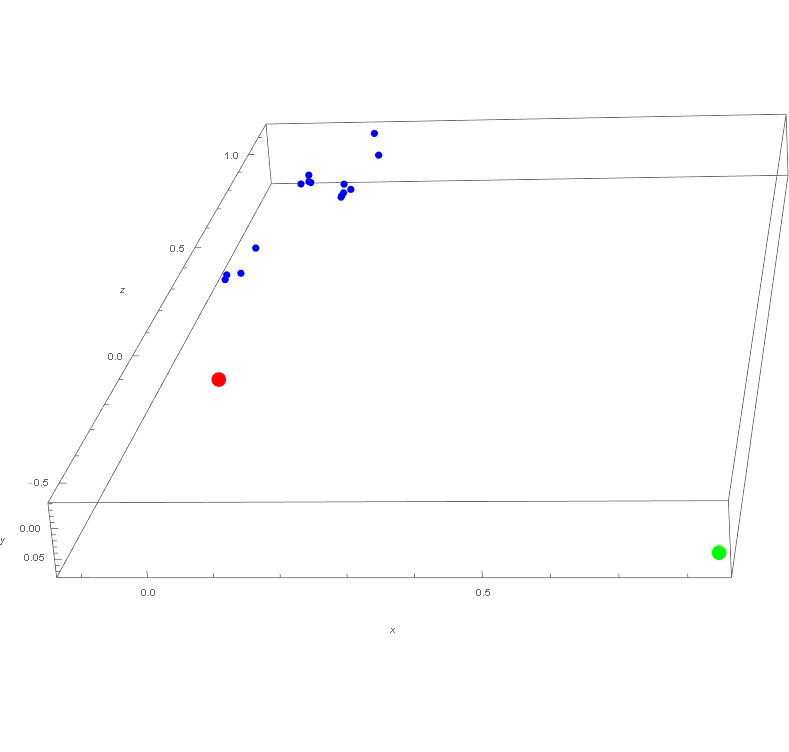
\includegraphics[width=\linewidth]{images/reconstructed_Points_Same_Resolutions.png}
	\caption{Rekonstruierte Szene, unskaliert in Pixeleinheiten}
	\label{fig:awesome_image1}
	\endminipage\hfill
	\minipage{0.48\textwidth}
	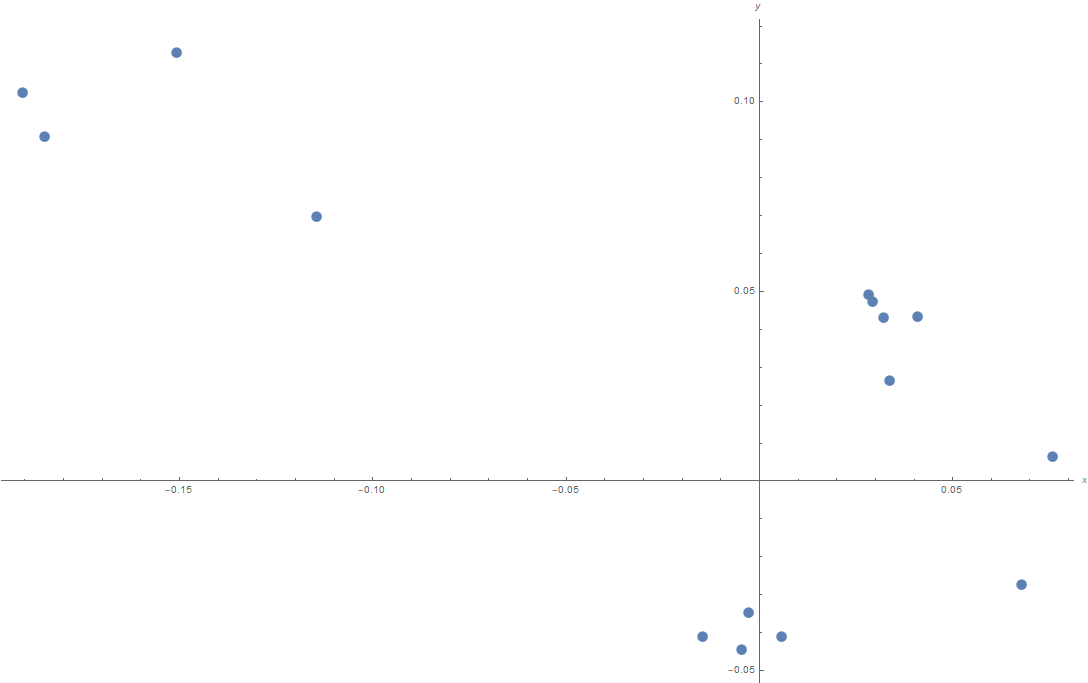
\includegraphics[width=\linewidth]{images/reconstructed_Points_Same_Resolutions2D.png}
	\caption{Rekonstruierte Szene, unskaliert, in Pixeleinheiten und in einem 2D-Plot geschrieben}
	\label{fig:awesome_image2}
	\endminipage\hfill
	%	\caption{Die mit dem \textit{SURF}-Algorithmus gefundenen Punkte sind mit den gelben Ziffern im Bild gekennzeichnet}
\end{figure}

%\begin{minipage}{\linewidth}
%	\centering
%	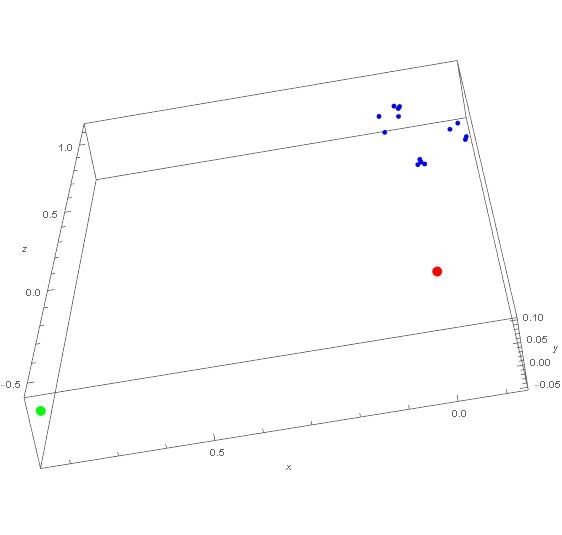
\includegraphics[width=.8\linewidth]{images/result_DetectedmathematicaPointsDifferentResolutions.png}
%	\captionof{figure}{Frafische Darstellung der optimalen Punkte $\hat{m}$ und $\hat{m'}$}
%\end{minipage}\\

%\subsection{andere Ansätze für Triangulationsverfahren}



